%---------- Sexto Capítulo: Resultados ----------
\chapter{Resultados}
\label{chap:result}
% TODO: introduzir a seção de resultados

\section{Metodologia Empregada}

% TODO: escrever texto e referencias as figuras
A metodologia empregada mencionada no capítulo \ref{metod} se mostrou bem eficiente ao longo do projeto.
A arquitetura do projeto possibilitou o desenvolvimento distribuído entre os integrantes, o que acelerou o processo de implementação efetiva do software.
Aliado a isto, utilizou-se a ferramenta GitHub, a qual facilitou ainda mais a metodologia empregada, já que tal ferramenta além de utilizada para controle de versionamento de código, forneceu meios para estabelecimento de metas e estatísticas de desempenho de cada desenvolvedor, técnicas fundamentais para gerenciamento do projeto.

Uma das estatísticas geradas é a evolução do número de linhas de código do projeto ao longo do tempo de desenvolvimento, mostrada na figura \ref{fig:linesofcode}.

\begin{figure}[!htb]
	\centering
	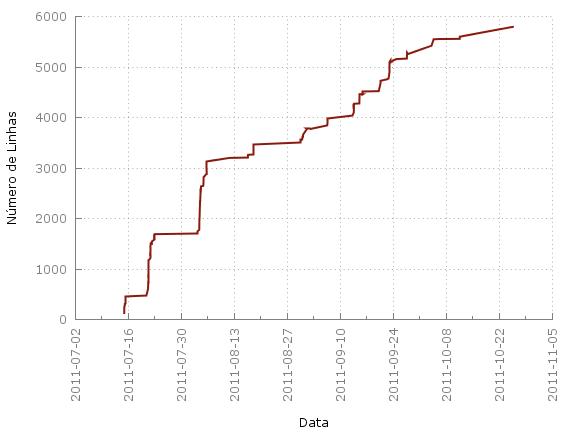
\includegraphics[width=0.7\textwidth]{./plots/lines_of_code.png}
	\caption[Evolução do número de linhas de código do projeto]{Evolução do número de linhas de código do projeto ao longo do processo de desenvolvimento}
	\fonte{Autoria Própria}
	\label{fig:linesofcode}
\end{figure}

Ao se observar a figura, percebe-se que a implementação efetiva do projeto foi iniciada dia 14 de julho e terminada em 25 de outubro do ano de 2011 com cerca de 6000 linhas de código. O maior salto de produtividade deu-se entre 24 de julho e 9 de agosto, período o qual foram criadas e implementadas grande parte das entidades do \emph{Core} do sistema. 

\begin{figure}[!htb]
	\centering
	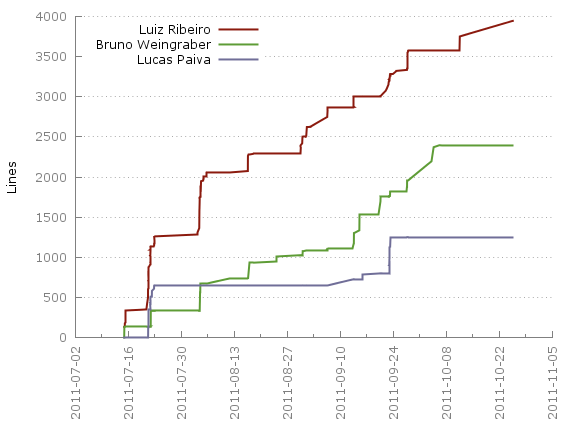
\includegraphics[width=0.7\textwidth]{./plots/lines_of_code_by_author.png}
	\caption[Evolução do número de linhas de código por programador]{Evolução do número de linhas de código do projeto por programador ao longo do processo de desenvolvimento}
	\fonte{Autoria Própria}
	\label{fig:linesofcodebyauthor}
\end{figure}

\begin{figure}[!htb]
	\centering
	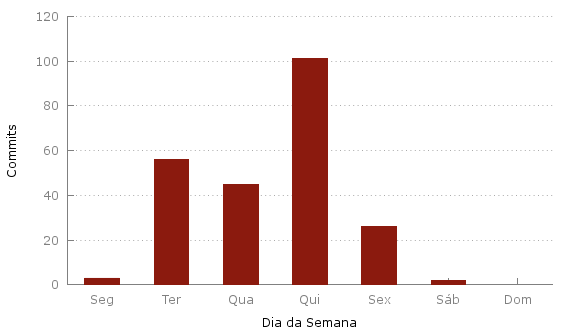
\includegraphics[width=0.7\textwidth]{./plots/day_of_week.png}
	\caption[Número de \emph{commits} por dia da semana]{Número de \emph{commits} por dia da semana}
	\fonte{Autoria Própria}
	\label{fig:dayofweek}
\end{figure}

\begin{figure}[!htb]
	\centering
	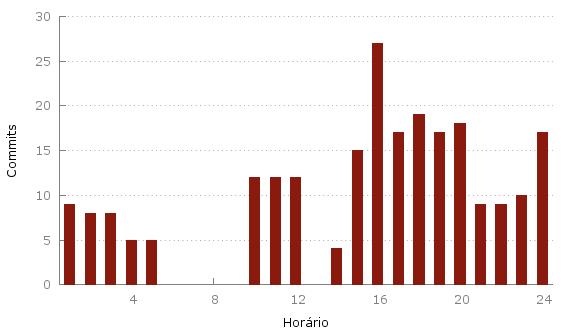
\includegraphics[width=0.7\textwidth]{./plots/hour_of_day.png}
	\caption[Número de \emph{commits} por horário]{Número de \emph{commits} por horário}
	\fonte{Autoria Própria}
	\label{fig:hourofday}
\end{figure}

\section{Performance do Sistema}

Como métrica para analisar a performance do sistema, optou-se por utilizar testes de \emph{stress} no \emph{Web Service}, ou seja, executar uma série de consultas simultaneamente e avaliar o impacto no tempo de resposta do mesmo.

Para tanto, foram realizados testes com o auxílio da ferramenta ApacheBench \cite{apachebench}.
Os testes foram executados em um único servidor com processador Intel{\textsuperscript\textregistered} Xeon{\textsuperscript\textregistered} X3450 de 2.67GHz e 2GB de memória RAM.
O servidor HTTP utilizado para hospedar a aplicação foi o Jetty, assim como descrito no Apêndice \ref{ape:guia}.

Tendo em vista a dificuldade que a equipe teve de obter informações de transporte público para cidades brasileiras, todos os testes utilizaram a base de dados do Bay Area Rapid Transit (BART), da cidade de São Francisco, Califórnia.
Esta base de dados é composta por 48 \emph{Stops}, 13 \emph{Routes}, cerca de 30 mil \emph{StopTimes} e 1500 \emph{Trips}.
% TODO: esse é o melhor jeito de dizer o tamanho da base de dados usada?

Foram executados cinco testes, sendo cada um destes composto por 1000 requisições.
O primeiro dos testes correspondeu à execução de todas as requisições sequencialmente, uma por segundo.
O segundo dos testes foi realizado com duas requisições concorrentes por segundo e, os demais testes, foram compostos por 5, 10 e 20 requisições por segundo.
O impacto do aumento do número de requisições concorrentes pode ser acompanhado através da Figura \ref{fig:response}, a qual apresenta o tempo de resposta para cada uma das requisições feitas nos testes descartando a latência da rede.

\begin{figure}[!htb]
	\centering
	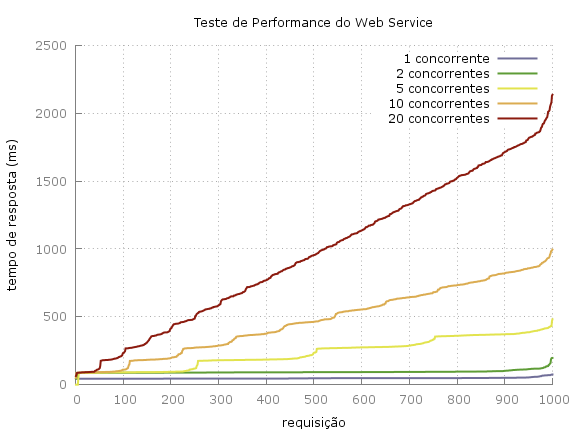
\includegraphics[width=0.7\textwidth]{./plots/stresstests/out.png}
	\caption[Tempo de resposta do \emph{Web Service}]{Tempo de resposta do \emph{Web Service} em função do número de requisições}
	\fonte{Autoria Própria}
	\label{fig:response}
\end{figure}

A partir do gráfico apresentado na Figura \ref{fig:response} é possível notar que, sob as condições propostas para o experimento, o serviço foi capaz de atender todas as requisições sequenciais em menos de 100 ms.
No teste de 2 requisições concorrentes por segundo, o serviço foi capaz de atender todas as requisições em menos de 200ms.
Para os testes de 5, 10 e, principalmente, 20 requisições concorrentes por segundo, as últimas requisições tiveram um tempo de resposta significativo, sendo em alguns casos necessários pouco mais de 2 segundos para responder a requisição de um cliente.

Apesar da aparente ruim performance no teste com 20 requisições concorrentes, deve-se levar em conta que para este teste foi utilizado apenas um servidor.
Para melhorar a performance do sistema em um ambiente com uma grande quantidade de requisições concorrentes, é possível utilizar diversos servidores e utilizar um mecanismo de escalonamento, de forma que as requisições sejam alocadas aos servidores que possuem mais tempo de CPU livre no momento, consequentemente minimizando o tempo de resposta.
Vale notar também que o caso de 20 requisições por segundo é um teste de \emph{stress} do sistema, o que não corresponde necessariamente à um caso de uso real.

\section{Considerações}

% TODO
